\documentclass[authoryear,11pt]{elsarticle}
	\usepackage[left=2.5cm, right=2.5cm,top=4cm, bottom=4cm]{geometry}

\usepackage{amsmath}
\usepackage{float}
\usepackage{verbatim}
\usepackage[american]{babel}
\usepackage{multirow}
\usepackage{setspace}

% ---------- watermark -----------
\usepackage[firstpage]{draftwatermark}
\SetWatermarkAngle{0}
\SetWatermarkFontSize{0.25cm}
\SetWatermarkVerCenter{1.15cm}
\SetWatermarkLightness{0.5}
\SetWatermarkHorCenter{14cm}
\SetWatermarkText{\shortstack[l]{
Voorspoels, W., Navarro, D. J., Perfors, A., Ransom K. and Storms, G. (2015). \\
How do people learn from negative evidence? Non-monotonic generalizations and \\
sampling assumptions in inductive reasoning. Cognitive Psychology, 81, 1-25 \\
http://dx.doi.org/10.1016/j.cogpsych.2015.07.001
}}
\SetWatermarkScale{1}
% -------------------------------

\newcounter{quotecount}
\newcommand{\MyQuote}[1]{\vspace{.5cm}\addtocounter{quotecount}{1}%
     \parbox{13cm}{\em #1}\hspace*{1cm}(\arabic{quotecount})\\[0cm]\vspace{.5cm}}

\begin{document}

\begin{frontmatter}

\title{How do people learn from negative evidence? Non-monotonic generalizations and sampling assumptions in inductive reasoning}

\journal{}

\author[leuven]{Wouter Voorspoels\corref{cor1}}
\ead{wouter.voorspoels@ppw.kuleuven.be}

\author[adelaide]{Danielle J. Navarro}
\ead{d.navarro@unsw.edu.au}

\author[adelaide]{Amy Perfors}
\ead{amy.perfors@unimelb.edu.au}

\author[adelaide]{Keith Ransom}
\ead{keith.ransom@adelaide.edu.au}

\author[leuven]{Gert Storms}
\ead{gert.storms@ppw.kuleuven.be}


\cortext[cor1]{Corresponding author}

\address[leuven]{Department of Psychology, University of Leuven, Belgium}
\address[adelaide]{School of Psychology, University of Adelaide, Australia}



	\begin{abstract}
A robust finding in category-based induction tasks is for positive observations to raise the willingness to generalize to other categories while negative observations lower the willingness to generalize. This pattern is referred to as monotonic generalization. Across three experiments we find systematic non-monotonicity effects, in which negative observations raise the willingness to generalize.
Experiments 1 and 2 show that this effect emerges in hierarchically structured domains when a negative observation from a different category is added to a positive observation. They also demonstrate that this is  related to a specific kind of shift in the reasoner's hypothesis space. Experiment 3 shows that the effect depends on the assumptions that the reasoner makes about how inductive arguments are constructed. Non-monotonic reasoning occurs when people believe the facts were put together by a helpful communicator, but monotonicity is restored when they believe the observations were sampled randomly from the environment.\\ \\
	{\it Keywords}: inductive reasoning, relevance, negative evidence, sampling assumptions, Bayesian inference
	\end{abstract}

\end{frontmatter}

\newpage

\section{Introduction}

Imagine you are a citizen in classical Greece. As usual, your friend Zeno is arguing on logical grounds that kangaroos can never outrun tortoises. Tired of having the same discussion over and over again, you run home to fetch your partner's tortoise, and in front of an enthusiastic crowd you race many other animals against it. Your neighbor's chicken, Diogenes' dog, the baker's horse and the local pig all beat the tortoise. You cheer, but Zeno insists that this does not logically dictate that kangaroos would beat tortoises. He then proposes to race his snail, the innkeeper's two-legged cat and an elderly Achilles, all of which lose. At the end of the day the tortoise dies of exhaustion and everyone goes home unsatisfied, realizing that due to the absence of kangaroos in classical Greece, the discussion will continue for years to come.

As this example shows, inductive reasoning has its limits. The main problem faced when making inferences on purely empirical grounds is that our data are often incomplete and our conclusions therefore uncertain \citep{Hume1739}. Whenever perfect evidence is lacking, making an inductive leap from known to unknown cases is unavoidable. In most cases the inductive leap is guided by \textit{similarity}. Consider the following category-based induction problem based on \citet{Rips1975}. The goal of the problem is to infer whether the conclusion under the solid line is  true, given the observation of the premise above the line.

\MyQuote{Premise: Tortoises have sesamoid bones\\[-5pt]
\rule[0pt]{250pt}{1pt} \\[-2pt]
Conclusion: Kangaroos have sesamoid bones}

\noindent
Without knowing anything else about sesamoid bones, acceptance of the conclusion is crucially dependent on the similarity between tortoises and kangaroos. Because properties are more readily projected between similar objects, similarity lies at the heart of most models of inductive inference \citep{Heit1998bay, Bloketal2007, Hayesetal2010, Medinetal2003, Oshersonetal1991, Oshersonetal1990, Sloman1993, Smithetal1993, Rips1975, Shepard1987}. As a result, if the premise had instead been that wallabies (rather than tortoises) have sesamoid bones, we would have been more likely to infer that kangaroos have them too. The same principle holds when the observation is negative rather than positive, but the outcomes are reversed. If told that wallabies {\it do not} have sesamoid bones, we would be very likely to reject the claim that kangaroos have sesamoid bones due to the perceived similarity between wallabies and kangaroos.

A simple prediction follows: there should be a monotonic relation between the number and sign of observations and the strength of an inference. As more objects with a property are observed, conclusions should be judged more likely (see, e.g., \citealt{Hayesetal2010, Heit2000, Lopez1995, Oshersonetal1990}). Conversely, as objects are observed that do not have the property, the judged likelihood of a conclusion should decrease. The magnitude of the shift depends critically on the extent of the similarity, but the direction depends on the ``sign'' of the observation.

The prediction of monotonicity is robustly supported by experimental evidence \citep{Oshersonetal1990, Oshersonetal1991, Smithetal1993}, but violations do occur \citep{Heussenetal2011, KalishLawson2007, Medinetal2003, Oshersonetal1990}. Our goal in this paper is to investigate when and why these violations arise, in particular when negative evidence is involved. First, we show empirical evidence of non-monotonic generalization on the basis of negative observations. Second, we present and test a theoretical analysis suggesting that assumptions regarding the selection of the observations play a crucial role in the emergence of non-monotonic generalization. Before describing our experiments, we begin with an overview of previous work and an explanation of our theoretical approach.

\subsection{When do negative observations support a conclusion?}

While the general tendency is for negative observations to weaken conclusions \citep{Oshersonetal1991}, in certain problems they can elicit a rise in willingness to generalize \citep{KalishLawson2007,Heussenetal2011}. For example, \citet{Heussenetal2011} presented participants with arguments like the following:

\MyQuote{Mozart's music elicits alpha waves in the brain\\
Metallica's music \textbf{does not} elicit alpha waves in the brain\\[-5pt]
\rule[0pt]{250pt}{1pt} \\[-2pt]
Bach's music elicits alpha waves in the brain
}

\noindent
People considered arguments like the above, which included a negative observation as well as a positive one, as stronger than the argument that only presented the positive observation. This violates the monotonicity prediction. Similarly, \citet{KalishLawson2007} provided evidence for violations using implicit negation, in which negative observations are implied based on the presence of an incompatible property. That is, participants were given arguments like the following:

\MyQuote{This wolf has bunit ears \\
This lion has liko ears\\[-5pt]
\rule[0pt]{250pt}{1pt} \\[-2pt]
This other wolf has bunit ears.
}

\noindent
This argument is rated as stronger than one that does not contain the information about the lion, suggesting that the effect arises even from indirect negative evidence.

Why is monotonicity violated in these cases? One possibility is suggested by the similar structure of arguments (2) and (3). In both, the negative observation comes from a different subcategory than both the first observation and the conclusion. However, it still lies within a common superordinate category. In argument (2), the negative observation is an instance of {\it rock music} and the first premise and the conclusion are {\it classical music}. In argument (3), the negative observation is still a mammal, but is not a member of the subcategory of {\it wolves}. In both cases we see negative observations from outside the category facilitating generalization within the category. This pattern makes sense if people assume that negative observations identify how far one should extend the property. Under such an assumption, the negative observation provides strong evidence for where the boundary actually lies.

More generally, these violations of monotonicity point to the necessity of considering that other mechanisms  besides similarity may bear on inference. One possibility is that negative observations can point the reasoner to a relevant dimension for inference \citep{Heussenetal2011, Medinetal2003}. Under this theory, the negative observation in the ``alpha waves'' argument highlights a commonality between Mozart and Bach that is not shared by Metallica. This implies that the property is shared by all classical music. According to relevance theory, people pick up on the relevance of {\it classical music} because the category-based induction task implies an act of communication that is made in a pragmatically cooperative context. Viewed in terms of the similarity-coverage model of category-based induction \citep{Oshersonetal1990}, the effect of adding the not-Metallica premise might be captured by shifting the reference category from a default choice of {\it music} to the hierarchically lower {\it classical music}. Since the latter category is better covered by the positive premise, it contributes positively to the strength of the argument. Although sensible, this mechanism has some severe problems from an explanatory perspective. Specifically, it contains no explanation for {\it why} the reasoner should shift the reference category in this way. Neither -- to foreshadow our empirical findings -- does it distinguish between cases where relevant negative evidence is generated from a helpful teacher, versus when random negative evidence is generated by the world.

This discussion raises several questions. Does the inclusion of negative evidence really act to focus the reasoner's attention on a particular category? Is the effect generally found in arguments that have the hierarchical category structure outlined above? Is the effect dependent on pragmatic assumptions made by the reasoner? If so, can those assumptions be changed? Is there a formal explanatory framework that can link the intuitive ideas about relevant negative evidence to specific predictions about reasoning? Our main goal in this paper is to address these questions, and to that end it is useful to consider the logic by which negative data can have evidentiary value within inductive inference.

\subsection{Why might negative observations support a conclusion?}

A classic argument for the informativeness of negative evidence is due to \citet{Hempel1945}. Suppose we observe that Carnap's wolf has bunit ears, and we agree that this provides inductive support for the conclusion that all wolves have bunit ears. The claim made by the conclusion is formally equivalent to the claim that all non-bunit eared things are not wolves.\footnote{If the original claim is $W \rightarrow B$, then $\neg B \rightarrow \neg W$ follows from the law of contraposition, and vice versa.} Now suppose we learn that Turing's lion has liko ears. Turing's lion is a non-bunit-eared non-wolf, and is consistent with the second version of the claim in precisely the same sense that Carnap's bunit-eared wolf is consistent with the first version of the claim. If one observation is informative, so is the other.

The difficulty with accepting this argument is that it is too general: people do not usually view negative observations as being anywhere near as informative as positive ones. This is not captured by the logic of Hempel's argument, which not only implies that Turing's lion is informative about wolves; it also implies that seeing a pair of green shoes is just as useful as seeing a black raven when trying to test the hypothesis that ``all ravens are black'' \citep[see, e.g.,][]{Nickerson1996}.

A probabilistic approach to reasoning resolves the concern raised by Hempel's analysis. The standard Bayesian answer was proposed by \citet{Good1960}, and it emphasizes the importance of frequency. The knowledge that very few things are ravens makes a black raven informative, whereas the knowledge that most things are not black makes non-black non-raven far less informative. Variations on this theme are commonplace in Bayesian analyses of human inductive reasoning, in which a relationship between size, frequency and informativeness appears in many different contexts \citep[e.g.][]{OaksfordChater1994,NavarroPerfors2011,NavarroPerfors2010,TenenbaumGriffiths2001,KlaymanHa1987}. These findings have been put forth to argue for the superiority of positive evidence over negative evidence in guiding inductive reasoning. However, while positive evidence is generally found to be more informative than negative evidence, the probabilistic view still provides scope for finding negative evidence useful.

How does negative evidence become informative within a probabilistic framework? The task facing a learner is to update her beliefs about the extension of a feature as she makes observations of objects with or without the feature \citep{Heit1998bay, TenenbaumGriffiths2001}. Bayes' theorem can be used to describe how the learner should update her hypotheses $h$ about which objects contain the feature $f$ in light of a negative observation $d^-$:

\begin{equation}
P(h_i=f|d^-) \propto P(d^-|h_i) P(h_i=f)
\label{eq:bayes}
\end{equation}

\noindent
Within this framework, beliefs are revised by combining the prior belief in a hypothesis $P(h_i=f)$ with the probability of a particular negative observation given that hypothesis $P(d^-|h_i)$, referred to as the likelihood. For our purposes, it is the likelihood that is of critical importance insofar as it acts as a theory about how the observations came to be. Facts that appear in an opinion piece in a newspaper have a very different provenance to the same facts when they arise as the result of a google search on the topic. Within the Bayesian framework, the learner's theory on how the facts were selected matters: different theories about the origin of the argument will lead to different conclusions, even when the same evidence is presented \citep[see also][]{Shaftoetal2012}.

To see how this works, consider the simplest theory a learner might entertain, known as \textit{weak sampling}. This theory assumes that a premise is constructed by selecting an item at random from all possible objects in the domain, and then identifying whether it possesses the property of interest. Such a theory is most appropriate in a naturalistic context where observations are made in a haphazard fashion. Under weak sampling, the chance of making observations about kangaroos, tortoises or centipedes is entirely independent of whether they have sesamoid bones. Formally, the probability of learning that item $d$ does not possess the property of interest (which we denote $d^-$) is given by:

\begin{equation}
P(d^- | h) \propto \left\{ \begin{array}{cl} 1 & \mbox{ if } d \notin h \\ 0 & \mbox{ if } d \in h \end{array} \right.
\label{eq:strong}
\end{equation}

With this as the underlying theory of the data generating process, observing that centipedes do not have sesamoid bones has only one effect: it falsifies those hypotheses that entail centipedes having sesamoid bones. Critically, it does not alter the relative degree of belief in any pair of hypotheses $h_1$ and $h_2$ that are  consistent with the negative observation. According to this model, $d^-$ has no systematic ability to strengthen conclusions.\footnote{It is in fact {\it possible} for a negative observation to increase generalization, if it just happens to be the case that the falsified hypotheses were less likely to be consistent with the conclusion than the unfalsified hypotheses. Overall, though, there is no reason to expect any {\it systematic} effect if the learner adopts this theory. Moreover, it would require salient hypotheses with cross-cutting extensions, instead of hierarchically structured hypotheses considered in this paper.}

More sophisticated sampling theories make different assumptions about how the argument was put together, and therefore license different generalizations. For instance, in {\it strong sampling}, positive observations are selected only after conditioning on the true extension of the property. For a negative observation $d^-$ it is assumed that the person constructing the argument deliberately {\it chose} to provide a negative observation, and then selected an example randomly from the set of items that are not in the property's extension. For a domain that consists of $n$ items, the probability that the negative item is chosen to be $d^-$ under strong sampling is

\begin{equation}
P(d^- | h) = \left\{ \begin{array}{cl} \frac{1}{n-|h|} & \mbox{ if } d \notin h \\ 0 & \mbox{ if } d \in h \end{array} \right.
\label{eq:negstrong}
\end{equation}

\noindent where $|h|$ denotes the number of items that belong to the hypothesis $h$.

Later in the paper we propose a much more sophisticated theory in which the reasoner takes account of the social and pragmatic factors involved in constructing an argument, but even this simple model makes an important qualitative prediction: negative evidence should cause people to revise their beliefs to favor the {\it largest} categories that exclude the negative observation. To see why, consider two hypotheses, $h_1$ and $h_2$, which the reasoner considers equally plausible before any evidence is given, so $P(h_1=f) = P(h_2=f)$. The learner is then told that item $d$ does not possess the property of interest. If both hypotheses are consistent with this evidence, weak sampling does not lead to any change in the reasoner's belief. In contrast, if she adopts the strong sampling view, the posterior odds ratio for $h_1$ versus $h_2$ is now given by:

\begin{equation}
\frac{ P(h_1 | d^-) }{ P(h_2 | d^-) } = \frac{ P( d^- | h_1 )}{ P( d^- | h_2 ) } \times \frac{ P(h_1) }{ P(h_2) } = \frac{n-|h_2|}{n-|h_1|}
\label{eq:hsize}
\end{equation}

\noindent This expression is greater than 1 if and only if $|h_1| > |h_2|$, indicating that the reasoner revises their belief to prefer the larger hypothesis.\footnote{It is also worth noting that if $|h_1|$ and $|h_2|$ are both small relative to $n$, the {\it magnitude} of the belief revision towards the large hypothesis is much smaller than the corresponding belief towards the small hypothesis that a positive observation provides. In other words, the strong sampling model still reproduces the critical feature of Good's \citeyear{Good1960} solution to the \citet{Hempel1945} paradox, namely that positive evidence is more powerful than negative evidence. While not directly relevant to the topic of our paper, this behavior is important to note, insofar as there is little value in considering theories that cannot reproduce the superiority of positive evidence under typical conditions.}

As this example illustrates, a reasoner does not need to have a very complicated theory of how inductive arguments are constructed in order to produce a pattern of belief revision strikingly different from the falsificationist logic that underpins weak sampling. Nor does it take a very complicated theory to predict a systematic effect in which negative evidence can strengthen conclusions. Later in the paper we show not only that this prediction is borne out, but also that our data suggest that human reasoning reflects a much more sophisticated theory of how arguments are constructed.

\subsection{Structure of the paper}

We present three experiments in this paper. In all three, people judge that a conclusion is more likely given a certain negative observation in a hierarchically structured argument. Experiments 1 and 2 include a concurrent hypothesis generation task, which suggests that non-monotonic generalization correlates with the specific shift in the hypothesis space suggested by the preceding analysis: namely, the largest hypothesis still consistent with the observations gains a disproportionate degree of belief when the negative observation appears.
Finally, Experiment 3 explicitly tests the prediction that non-monotonicities depend on the reasoner's theory of how arguments are constructed. It demonstrates that the empirical effect vanishes when participants are convinced that the data are weakly sampled, but remains when they believe that the argument consists of facts assembled by a helpful teacher.

\section{Experiment 1}

The goal of this experiment is to evaluate how generalizations are affected by the structure of the hypothesis space and location of negative evidence relative to that structure. In addition to directly measuring generalization we also ask participants to generate hypotheses about the true extension of the feature.

\subsection{Method}
\subsubsection{Participants}

Participants were 175 undergraduate psychology students at the University of Leuven (133 female) who volunteered for course credit. The average age was 18.45.

\subsubsection{Materials}

The inductive arguments used in the study were constructed with respect to a target category $T$, such as {\it music}. Items from this category could be drawn from one of two sub-categories ($T_1$ and $T_2$) such as {\it classical music} or {\it rock music}. Additionally, premises might be drawn from a contrast category $C$ (e.g., {\it nature sounds})\footnote{Contrast categories are mutually exclusive categories at the same level of abstraction that share a common superordinate. No implication of psychological contrast is intended.}. We constructed three different kinds of argument. In the {\sc baseline} condition, a single positive example from one of the subcategories was given, denoted ${T_1}^+$. For instance, participants might be told that Mozart's music elicits alpha waves. In the {\sc close negative} condition, they were provided with two premises, the baseline item plus a negative observation ${T_2}^-$ drawn from the other subcategory. In the music example, participants were told that Mozart's music does elicit alpha waves, but Metallica's music does not. Finally, in the {\sc distant negative} condition, the negative observation $C^-$ comes from a contrast category. Thus, in this condition, participants were told that Mozart's music elicits alpha waves, but the sound of a falling rock does not.  For all three conditions, we measured generalization by picking conclusion items from both target subcategories $T_1$ and $T_2$ as well as the contrast category $C$. The design is schematically illustrated in Figure~\ref{fig:exp1_itemstruc}.

To construct arguments we used 12 topics from \citet{Heussenetal2011}: music, painters, public figures, types of ships, types of glass, types of displays, water bodies, wind instruments, fruit, water birds, insects, polar animals. The properties to be generalized were designed to sound realistic but correspond to things that people were likely to have little or no knowledge about (e.g., \textit{contain lycopene, create conversion currents, elicit alpha waves in the brain}). Table~\ref{table:stimexp1} lists the premise and conclusion items for each topic.

\begin{figure}[p]
\begin{center}
\begin{tabular}{cc}
\raisebox{-2cm}{
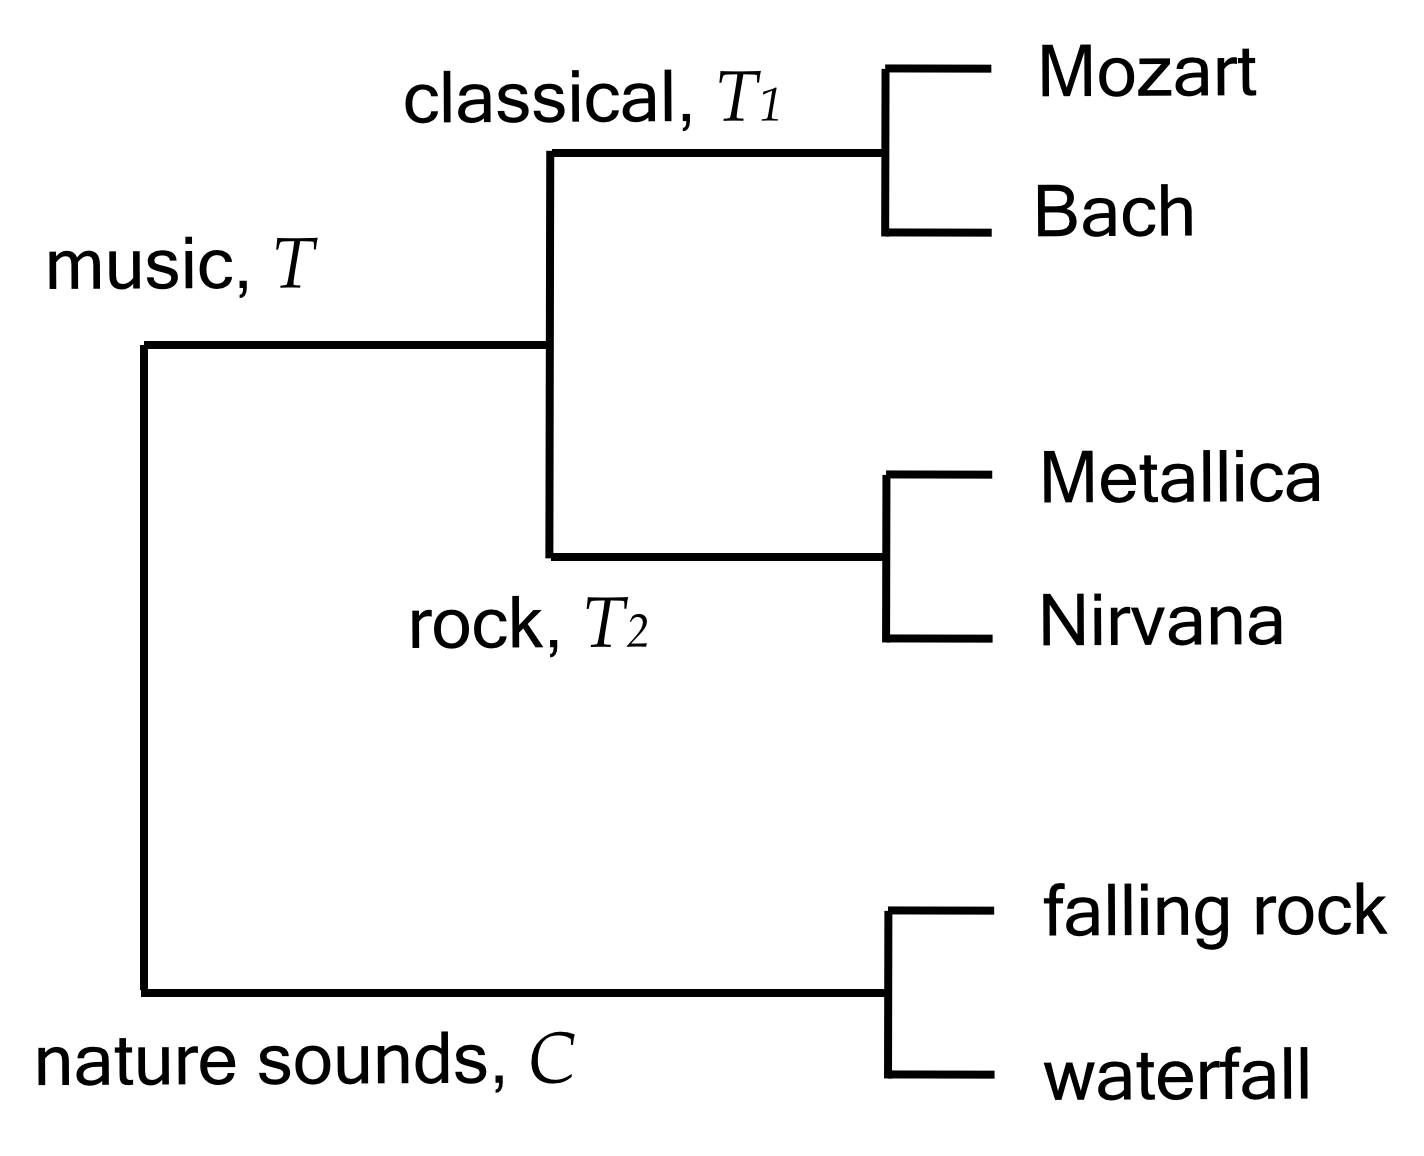
\includegraphics[width=6cm]{fig/exp1_itemstruc2.png}
}
\hspace{.5cm}
&
\footnotesize
\begin{tabular}{l|l}
%&& \multicolumn{3}{c}{conclusion item} \\
condition & premises shown  \\ \hline
{\sc baseline} & ${T_1}^+$  \\
{\sc close negative} & $\{{T_1}^+, {T_2}^-\}$ \\
{\sc distant negative} & $\{{T_1}^+, {C}^-\}$
\end{tabular}
\end{tabular}
\end{center}
%\vspace{-8mm}
\caption{\small A schematic representation of the structure of arguments when the target category $T$ is {\it music}. In the {\sc baseline} condition, participants are presented with a base premise consisting of a positive observation from subcategory $T_1$, in this case {\it classical music}. In the {\sc close negative} condition, a negative observation the other subcategory $T_2$ ({\it rock music}) is added. Finally, in the {\sc distant negative} condition the negative observation comes from the contrast category $C$, {\it nature sounds}. In all conditions, we obtain generalization judgments for items from categories $T_1$, $T_2$ and $C$.\normalsize}
\label{fig:exp1_itemstruc}
\end{figure}

\begin{table}[p]
\scriptsize
\caption{\small Premise and conclusion items for Experiment 1, translated from Dutch. Depending on the condition, the premise items could include positive examples from one subcategory of the target category ${T_1}^+$, the negative example from the other subcategory ${T_2}^-$, or the negative example from the contrast category $C^-$. The conclusion items were drawn from the same three categories, $T_1$, $T_2$ or $C$. The arguments were constructed with respect to 12 different topics, as shown below\normalsize}
\vspace{-2mm}
\label{table:stimexp1}
\vskip 0.12in
\begin{tabular}{|l|lll|lll|}
\hline
Topic & \multicolumn{3}{c|}{Premise items} & \multicolumn{3}{c|}{Conclusion items}\\
& ${T_1}^+$ &  ${T_2}^-$ & $C^-$ & $T_1$ &  $T_2$ & $C$\\
\hline
music 		&Mozart	    & $-$Metallica		& $-$falling rock	& Bach & Nirvana & waterfall\\
painters	&Rubens			& $-$Dali & $-$woodcarver & Van Eyck & Warhol & sculptor\\
public figures &actors& $-$librarians & $-$moles & politicians & programmers & pheasants\\
ships & freight ships & $-$hoverships & $-$cars & cruise ships & sail boats & rocks\\
glass & window glass	& $-$bottle glass & $-$art glass & car glass & drinking glass & jewelry glass\\
displays &	LCD   	& $-$television	& $-$paintings & plasma  & traffic signs & book page\\
water bodies &Atlantic&  $-$Lake Balaton & $-$mustard gas & Mediterranean & Silver Lake & olive oil\\
wind & flute & $-$guitar & $-$crying child&clarinet&violin& door\\
fruit & strawberries	& $-$bananas & $-$blades of grass & cranberries & apples & oak leaves\\
water birds	& ducks & $-$sparrows & $-$elephants & seagulls & blackbirds & camels\\
insects	& moths 		& $-$spiders & $-$lizards & flies & centipedes & goldfish\\
polar animals & polar bears & $-$deer & $-$sow bugs & penguins & parakeets & ants\\
\hline \multicolumn{7}{c}{ }
\end{tabular}
\end{table}

\subsubsection{Procedure}

The experiment was conducted via online survey. On each trial, participants were presented with a short vignette explaining a recent discovery related to the topic. The premise item(s) were presented to people as part of this vignette, and participants were asked to make a series of judgments related to the scenario.  In the {\it hypothesis generation} task they were asked to come up with a rule or hypothesis (one per vignette) that would explain the observations in the premises, and type their answer into a text box. In the {\it generalization} task that followed, they were presented with three different conclusion items in a random order, one each from categories $T_1$, $T_2$ and $C$, and asked to judge how likely it is that the item would have the property. Judgments were made by moving a slider along a continuous scale running from 1 to 100.

Each participant was presented with two practice arguments in order to make sure they understood the task, followed by 12 arguments presented in a random order, six of which pertained to the current study and the other six formed part of an unrelated study. Across the six scenarios relevant to the current experiment, all three premise conditions were each presented twice. The experiment took less than 20 minutes.

\subsection{Results: Generalization}

Responses to the generalization questions are plotted in Figure~\ref{fig:exp1me}, separately for the three premise conditions and the three conclusion types. Overall, the pattern of generalization is very sensible: in all conditions people were most willing to generalize a property to new members of the subcategory $T_1$ from which they have seen a positive example, less willing to generalize to the other subcategory $T_2$, and even less willing to do so to the more distant contrast category $C$.

The critical finding is the non-monotonic inference that occurs when we compare generalizations to the alternative subcategory $T_2$ (middle panel) in the {\sc distant negative} condition (light grey) to the {\sc baseline} condition (black). When given only a single positive example from the first subcategory $T_1$, participants believed that the property had a 35\% chance of generalizing to a member of the other subcategory $T_2$. But when they were also told that a member of the contrast category $C$ did not possess the property, the willingness to generalize to $T_2$ jumped to 54\%. This difference corresponds to a moderately large estimated effect size (Cohen's $d=.55$) and a Bayesian $t$-test applied to this pair of conditions produced a Bayes factor (BF) of approximately $10^9$:1 in favor of an effect.\footnote{Bayes factors were computed using the BayesFactor package in R \citep{BayesFactorManual}. Throughout our analyses we report only those Bayes factors immediately relevant to our findings, and as much as possible we report the simplest analysis we could. However, in our actual data analysis we always began with the full model for the data set as a whole, which in this case included crossed random effects for participant and topic and fixed effect terms for premise condition, following \citet{Baayenetal2008}. In all cases the more complicated analysis yielded the same conclusions as the simpler and more specific ones, so for the sake of readability we report only the relevant analyses.} Framed in terms of the {\it music} example, participants were more likely to conclude that Nirvana's music elicits alpha waves when they were told that the sound of falling rocks does not do so.

For generalizations to the base subcategory $T_1$, no such effect was found when the negative observation came from the nearby subcategory (BF = 9.9:1 in favor of no difference). Being told that Metallica's music does not elicit alpha waves had no influence on participants' willingness to generalize from Mozart to Bach. However, given that they were very willing to generalize within the base subcategory $T_1$ across all conditions (average generalization judgment of 72\%), it seems quite possible that a ceiling effect masked any effect in this condition, as the maximum average generalization score in all our experiments were around 75\%. Also, while the hypotheses generation task points to an increase in hypotheses regarding the subcategory $T1$ (e.g., classical music having the property) when adding a close negative premise, this increase seems, for the most part, due to falsification of the larger hypotheses (see Figure~\ref{rulegen}). As these larger hypotheses also contain the $T_1$ conclusion, one does not necessarily expect a strong non-monotonic effect on generalization judgments.

\begin{figure}[t!]
\begin{center}
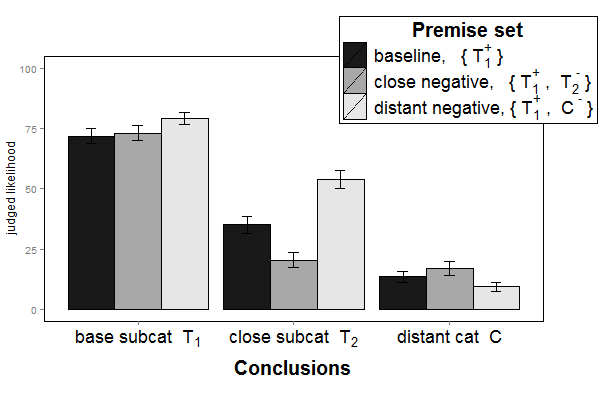
\includegraphics[trim=0cm 0cm 0cm 0cm, clip=true, scale=.5]{fig/exp1_gen_all.png}
\end{center}
\vspace{-8mm}
\caption{\small Average strength of belief in different conclusions in Experiment 1. Each bar plots the average judged probability that a property should be extended to a novel observation. Responses are broken down by the category to which the conclusion item belongs and by the premises that the participants saw. Conclusions could either belong to the subcategory $T_1$ from which the learner has seen a positive example, a close but different subcategory $T_2$ within the target category, and the distant contrast category $C$. The three premise types correspond to the {\sc baseline} condition in which only the positive example ${T_1}^+$ is observed, the {\sc close negative} condition in which the additional negative observation is ${T_2}^-$ and the {\sc distant negative} condition where it is from category $C^-$. Error bars show 95\% confidence intervals. The critical finding is the non-monotonicity effect in the {\sc distant negative} condition relative to {\sc baseline}: when presented with ${T_1}^+,C^-$ people are much more willing to generalize to the close subcategory $T_2$ than if only presented with ${T_1}^+$. \normalsize}
\label{fig:exp1me}
\end{figure}

\subsection{Results: Hypothesis generation}

In the hypothesis generation task, participants generated one hypothesis for each premise set they were presented with. The free responses were coded into types using the following scheme. The {\sc unique} type included answers indicating that the property was possessed only by the specific exemplar presented in the base premise (only Mozart). The {\sc subcategory} type included answers that extended the property to all members of the targeted base subcategory (classical music), as well as responses that concerned a subcategory that did not correspond to the targeted base subcategory (e.g., `soothing music').\footnote{ The question we want to answer is not whether participants shift belief to the hypothesis we had in mind, but whether they shift belief to larger hypotheses. Importantly, both {\sc subcategory} types comprise hypotheses that are subsets of, and therefore smaller than the category (music), but larger than the {\sc unique} hypotheses (Mozart's music).}  The {\sc category} level responses are those that cover the whole target category (music). Finally, {\sc superordinate} responses are those that extend the property to the higher level category (all sounds). The criterion for coding was the literal appearance of the intended terms: responses that were vague, ambiguous or crosscutting (e.g., ``some types of music'', ``calming sounds'') were coded as {\sc other} and not analyzed further. The latter group comprised 22\% of the responses (17\% in the {\sc baseline}, 21\% in the {\sc close negative} and 28\% in the {\sc distant negative} condition).

\begin{figure}[t]
\begin{center}
\includegraphics[trim=0cm -.5cm 0cm 0cm, clip=true, scale=.45]{fig/Exp1_hgen.png}
\end{center}
\vspace{-10mm}
\caption{\small Frequency distribution over the different kinds of hypothesis generated by participants, broken down by condition. See main text for an explanation of the coding scheme. Hypotheses that are inconsistent with the negative evidence are almost never generated (falsification occurs). When negative evidence is added, the relative degree of belief among non-falsified hypotheses shifts. Relative to the {\sc baseline} condition, the two {\sc negative} evidence conditions both show a redistribution of beliefs from small hypotheses towards the largest hypothesis consistent with the data. \normalsize}
\label{rulegen}
\end{figure}

The relative frequency of the different response types is shown in Figure~\ref{rulegen}, broken down by premise condition. In the {\sc baseline} condition, the responses reflect a preference for {\sc subcategory} hypotheses, with comparatively few people proposing that the property generalizes to the {\sc superordinate} level. Not surprisingly, providing negative evidence served a falsification role: in the {\sc distant negative} condition, the only category falsified was the {\sc superordinate} level, and accordingly the responses at that level dropped to near-zero frequency. In the {\sc close negative} condition, where the negative evidence came from a member of the target category, both the {\sc superordinate} and {\sc category} level hypotheses are falsified, and again those responses drop to near-zero frequency. As noted in the introduction, this falsification behavior is consistent with both the weak and strong sampling models.

The critical prediction of the strong sampling model is that when negative evidence is provided, the largest non-falsified category should show a disproportionate rise, relative to smaller non-falsified categories. The data provide two tests of this hypothesis. First, the ratio of {\sc subcategory} to {\sc unique} responses should be larger in the {\sc close negative} condition than in the {\sc baseline} condition, as participants should shift their beliefs to favor the target subcategory $T_1$ or another subcategory of the target category $T$. Secondly, when comparing the {\sc distant negative} condition to {\sc baseline} the relevant comparison is between the number of {\sc category} level responses and the number of responses that reflect a smaller category (i.e., either {\sc subcategory} or {\sc unique}), because participants should shift their beliefs towards the target category $T$. Visual inspection of Figure~\ref{rulegen} suggests that both effects occur.

The expected belief shifts are confirmed by Bayesian analyses. Using a custom Bayesian model\footnote{The null model assumes that the hypothesis generation probabilities are the same in all conditions, except insofar as hypotheses falsified by negative evidence drop to near zero probability and the others rise proportionally. The alternative model postulates that over and above this effect, some proportion of the belief shifts away from the smaller hypotheses to the largest non-falsified hypothesis.} implemented in JAGS we estimated the Bayes factor to be 48:1 in favor of a systematic shift. Over and above the expected rises due to falsification of the larger hypotheses that were inconsistent with the observation, the model estimated that in the {\sc close negative} condition 45\% of people's belief in {\sc unique} hypotheses was transferred to {\sc subcategory} hypotheses, and in the {\sc distant negative} condition 25\% of the belief in {\sc unique} and {\sc subcategory} hypotheses. However, the 95\% credible intervals for these were [23\%,62\%] and [2\%,51\%] so there is considerable uncertainty about the exact numbers and no clear evidence that the amount of belief change was actually different across these conditions.

Finally, to make sure that at the individual level the generation of a certain hypothesis was related to the generalization judgment, we conducted additional analyses, comparing the preferred mixed model of the generalization judgments with an ``augmented'' version including the hypothesis type as an additional categorical factor. The augmented model was clearly preferred , both for generalizations to the base subcategory (BF = 600.6:1) and generalizations to the alternative subcategory (BF = $8.2E+54$:1 ). This indicates that the type of hypothesis generated by participants mediated the relation between the premise set and their subsequent generalization judgment. To illustrate the mediation, the critical non-monotonic generalization to the alternative subcategory $T_2$ observed in the {\sc distant negative} condition, did hold for participants that generated the {\sc category} hypothesis, on average endorsing the generalization by 73\%, but not for participants that generated the {\sc unique} (average judgment: 27\%) or {\sc subcategory} (average judgment: 24\%) hypothesis.

\subsection{Discussion}

The generalization data from Experiment 1 provide good support for the idea that negative observations can strengthen people's belief in a conclusion in some situations. This is a clear violation of monotonicity consistent with earlier work  \citep{Heussenetal2011, KalishLawson2007}. Unlike \citet{Heussenetal2011} we did not detect non-monotonic generalizations in the {\sc close negative} condition, but this seems likely to be a ceiling effect. More tellingly, when we examine the hypotheses that people offered, we find evidence for belief revision that can {\it not} not be merely due to the falsification of alternative inconsistent hypotheses. Regardless of how distant the negative observation is from the positive one, we observe a shift in the relative degree of belief even among the non-falsified hypotheses. This shift is precisely the one predicted by the strong sampling model: people transfer belief to the largest consistent hypothesis.

\section{Experiment 2}

We have three motivations for Experiment 2. Our first goal is pseudo-replication. The effects in Experiment 1 were surprising to us in light of the usual finding of monotonicity, and we wanted to see if the effect could be reproduced in a similar experiment. Secondly, as highlighted in Table \ref{table:stimexp1}, the topics included in Experiment 1 are very diverse, and many are in domains (e.g., {\it types of glass}) that are rather atypical of the category-based induction literature. We wanted to perform a detailed replication focusing entirely on a domain that is highly typical of the existing literature: {\it animals} \citep{Coleyetal2004, Medinetal2003, Oshersonetal1990, Oshersonetal1991, Smithetal1993}.

Our third motivation emerges out of a consideration of the structure of the hypotheses involved. There is a sense in which the ``hierarchical'' structure to the arguments is something of an artifact of the way we constructed the stimuli. The domain of public figures is not naturally hierarchical, for instance, but a hierarchical structure arises because of the particular categories that we used to generate evidence. It is only through the specific choice of premises in Table~\ref{table:stimexp1} that the hierarchical structure in Figure~\ref{fig:exp1_itemstruc} arises. For the most part, we think this is actually a positive feature of the result, because it implies that the non-monotonicity arises due to the structure of the {\it argument} not the structure of the mental representations that people rely on. Even so, we felt it would also be sensible to check that the result appears when the hierarchical structure in the argument emerges more naturally from the hierarchical structure of the mental representation.

The structure underlying the arguments in Experiment 1 can be easily translated to the domain of animals: any member of an animal category, like mammals, can serve as base premise. We would expect non-monotonic generalization when a negative observation from a different animal category is added to the premise set. For example, observing that birds do not have a property while dogs do should increase generalization to another mammal, like a donkey (see Figure~\ref{fig:exp2_itemstruc}). Arguments for other animal categories can be formed in a structurally identical fashion.

\begin{figure}[t!]
\begin{center}
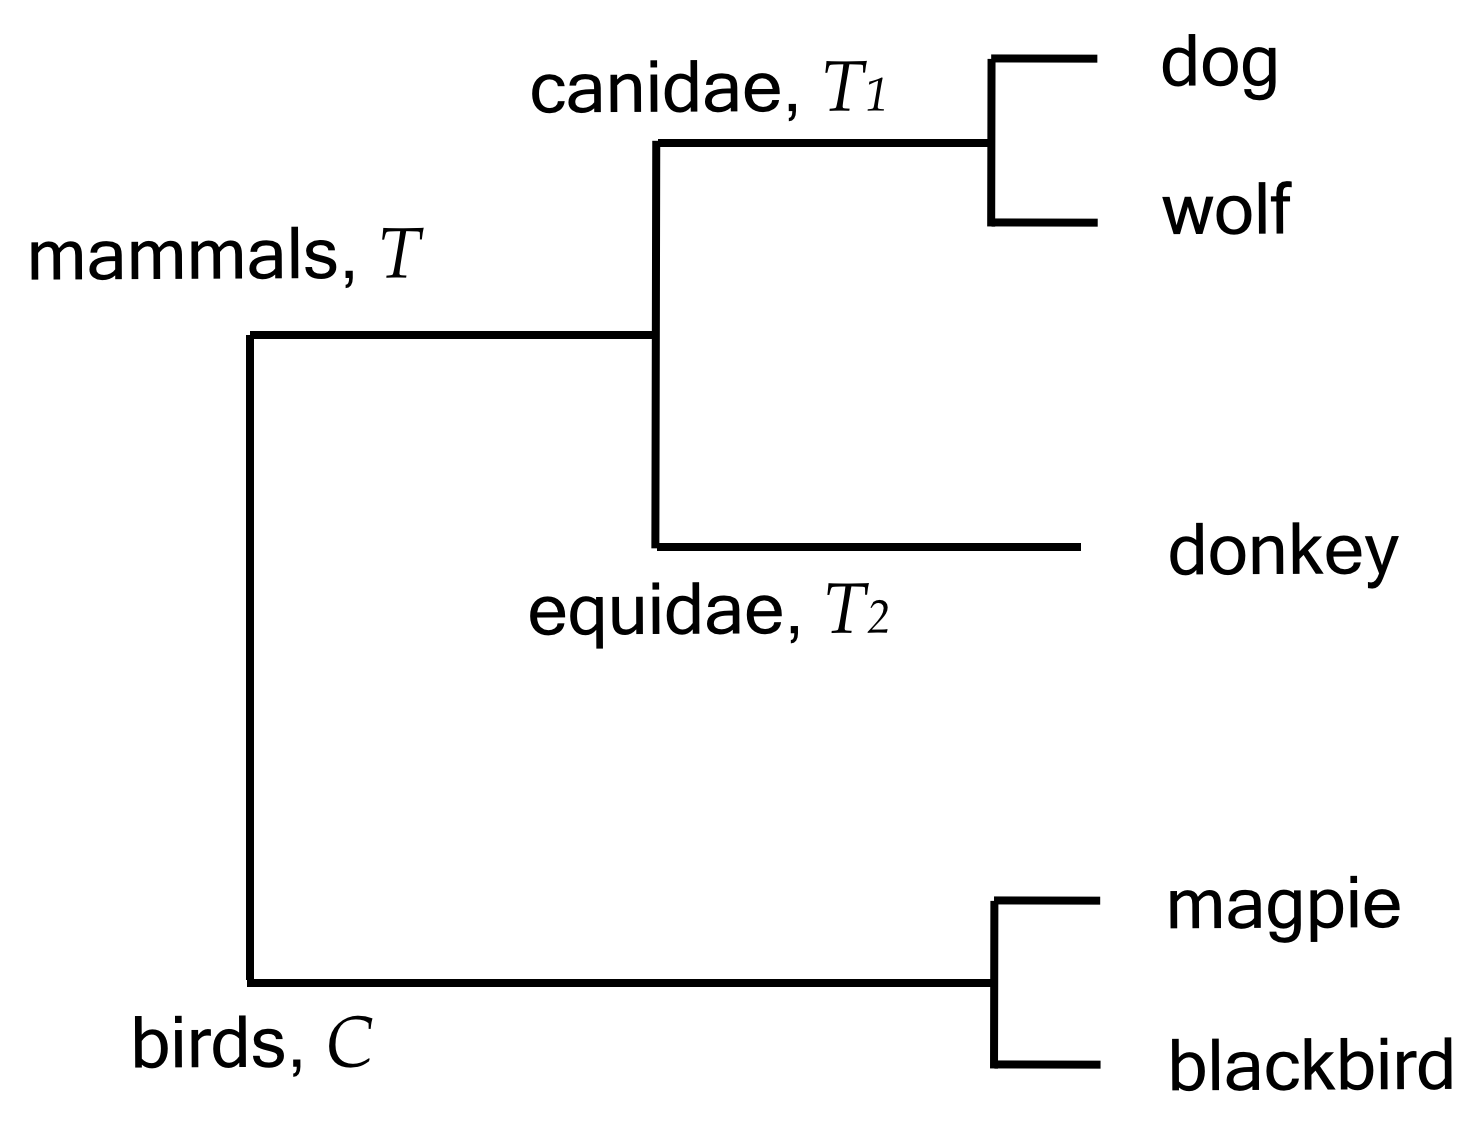
\includegraphics[width=6cm]{fig/exp2_itemstruc2.png}
\end{center}
\vspace{-8mm}
\caption{\small A schematic representation of the structure used in Experiment 2. In the {\sc baseline} condition a single positive example from the $T_1$ subcategory was presented (e.g., {\it dog}), and in the {\sc negative} condition this was supplemented with a negative observation from the contrast category $C$ (e.g., {\it magpie}). Generalizations to all three relevant categories were tested by presenting conclusion items from categories $T_1$, $T_2$ and $C$ (e.g., {\it wolf}, {\it donkey} and {\it blackbird})}
\label{fig:exp2_itemstruc}
\end{figure}

\subsection{Method}

\subsubsection{Participants}
Seventy-nine undergraduate psychology students at the University of Leuven (66 females) took part for course credit. The average age was 18.69 years.

\subsubsection{Materials}

We considered four arguments in the domain of animals, each one with a baseline premise from a different category: birds, fish, insects, and mammals. Following the same logic as Experiment 1, there was a {\sc baseline} condition that presented a single positive example from the base subcategory $T_1$. The {\sc negative} condition was analogous to the {\sc distant negative condition} from Experiment 1, in which participants were also shown a negative example from the contrast category $C$. We did not include an analog of the {\sc close negative} condition given that the effects were attenuated in that condition. As before, the conclusion items were drawn from both subcategories of the target category, $T_1$ and $T_2$, as well as from the contrast category $C$. The specific premises and conclusions used are listed in Table \ref{table:stimexp2}.

\begin{table}[t!]
\scriptsize
\begin{center}
\caption{Stimulus material used in Experiment 2 (translated from Dutch). Each argument was presented with the {\sc baseline} premise. In the {\sc negative} condition, a second negative premise from a different category (C) was also shown. Participants gave generalizations to all three conclusions.}
\label{table:stimexp2}
\vskip 0.12in
\begin{tabular}{|c|cc|ccc|}
\hline
 & \multicolumn{2}{c}{Premise items} & \multicolumn{3}{c|}{Conclusion items}\\
 \hline
area & ${T_1}^+$ &  $C^-$ &  $T_1$ & $T_2$ & $C$ \\
\hline
mammals & dog & -magpie & wolf & donkey & blackbird\\
birds	& crow & -tuna fish & raven & swan & halibot\\
fish	& salmon & -lizard & codfish & goldfish & snake\\
insects	& bee & -sparrow & ant & cricket & pigeon\\
\hline \multicolumn{6}{c}{ }
\end{tabular}
\end{center}
\end{table}

\subsubsection{Procedure}

The general procedure was identical to Experiment 1. Participants were first presented with the premise set and were asked to type in one hypothesis that, according to them, would explain the observation(s) in the premise set. Then they judged the likelihood of three conclusions in random order, each one generalizing the property to another animal from a different category or subcategory. To get accustomed to the procedure, the same practice argument was presented first.

Every participant was presented with all four arguments, two with the {\sc baseline} premise set and two with the {\sc negative} set. Half the participants saw the mammals and birds arguments in the {\sc baseline} condition and fish and insects in {\sc negative} condition, and the other half saw the arguments the other way around. To eliminate demand effects, four filler arguments were also constructed to diversify the premise sets and obscure our focus on negative observations.

\subsection{Results}

\begin{figure}[t]
\begin{center}
\includegraphics[scale=.45]{fig/Exp2_gen_all.png}
\end{center}
\vspace{-7mm}
\caption{\small Average willingness to generalize to various conclusion as a function of the premise set. Error bars depict the 95\% CI. As in Experiment 1, non-monotonic generalization can be observed when the conclusion item comes from a close subcategory (i.e. $T_2$) to the positive exemplar, and a negative observation from a contrast category $C$ is added. \normalsize}
\label{fig:Exp2_MainEffects}
\end{figure}

Participants' generalizations, plotted in Figure \ref{fig:Exp2_MainEffects}, reveal that the effect replicates well. The overall pattern of generalizations remains sensible and mirrors the results from Experiment 1. As with Experiment 1 the critical comparison is the one in the middle panel: people are more willing to generalize to the $T_2$ item ({\it donkey}) when the positive $T_1$ exemplar (i.e., {\it dog}) is augmented with a negative observation from the contrast category $C$ (i.e., not {\it magpie}). The effect size is slightly smaller than in the first experiment (Cohen's $d$ = 0.36), but the Bayesian $t$-test still finds moderate evidence (BF = 12:1) for an effect.

For the hypothesis generation task, we coded responses using the same scheme as Experiment 1 (18\% of responses did not fit the scheme in the {\sc baseline} condition, and 19 \% in the {\sc negative} condition), and the results are plotted in Figure~\ref{fig:Exp2_Hgen}. The main difference from Experiment 1 is that fewer hypotheses at the {\sc subcategory} level were generated: the majority of responses were at the {\sc category} level. Because of the simpler design of Experiment 2 and the fact that almost no {\sc superordinate} level responses were generated (meaning that we do not need to control for the falsification effect), the data analysis is much simpler than in Experiment 1. The question of interest is whether the proportion of {\sc category} level responses relative to {\sc unique} and {\sc subcategory} level responses is the same across conditions. In the {\sc baseline} condition the {\sc category} level responses outnumber the {\sc unique} and {\sc subcategory} responses by approximately 2:1, whereas in the {\sc negative} condition the ratio jumps to 6:1. A Bayesian test for the equality of proportions found strong evidence (BF = 10000:1) that a real difference exists.

As in experiment 1, we compared mixed models of of the effect of premise set on generalization scores with augmented models including the generated hypothesis type as an additional factor. We found that the type of hypothesis participants generated clearly mediated the relationship between premise set and generalization judgment, both for generalizations to the base subcategory $T_1$ (BF=$2.97E+14$ in favor of an augmented model) and to the alternative subcategory $T_2$ (BF=$1.19E+15$ in favor of an augmented model). To illustrate, participants generating a {\sc category} hypothesis in the {\sc negative} condition displayed non-monotonic generalization to the close subcategory $T_2$ (average generalization judgment of 75\%), contrary to participants generating a {\sc unique} (average judgment of 40\%) or {\sc subcategory} (average judgment of 32\%) hypothesis.

\begin{figure}[t]
\begin{center}
\includegraphics[trim=0cm 0cm 0cm 0cm, clip=true, scale=.45]{fig/Exp2_hgen.png}
\end{center}
\vspace{-7mm}
\caption{\small Relative frequency of generating different kinds of hypotheses as a function of the premise set. Each panel corresponds to one of the two premise set conditions. As in Experiment 1, adding negative evidence from a contrast category shifts people's beliefs towards the largest hypotheses (i.e. to the {\sc category} level) consistent with the negative datum.\normalsize}
\label{fig:Exp2_Hgen}
\end{figure}

\subsection{Discussion}

Taken together, Experiments 1 and 2 provide evidence that non-monotonic generalization can result from negative observations. Our results further suggest that given a hierarchically structured argument, negative observations can result in belief redistribution in favor of the largest hypothesis that is consistent with the observations. That is, people do not merely use negative evidence for falsification purposes, they redistribute belief among the data-consistent hypotheses in precisely the fashion predicted by a simple Bayesian model of inductive reasoning.

In Experiment 2, we observed a smaller effect size of the addition of a distant negative observation than in Experiment 1. This seemed mainly due to a larger willingness to generalize to the alternative subcategory even in the {\sc baseline} condition (on average 56\%, as compared to 35\% in Experiment 1). This, in turn,  is arguably due to substantially more participants projecting the property to the category level(e.g., mammals), increasing their willingness to generalize to $T_2$ in the {\sc baseline} condition  .

\section{What do people assume about how arguments are constructed?}

One of the central features of the probabilistic approach to human reasoning is that inductive inferences are constrained not only by the data and by the reasoner's priors, but also by their theory of how the argument was constructed. As we discussed in the introduction, these theories have a critical role to play in how people assess the value of negative evidence. If the learner believes that the premises in an argument consist of a random set of true facts about the world, a {\it weak sampling} theory is appropriate, and the belief revision is restricted to falsification of inconsistent hypotheses. However, the empirical data from Experiments 1 and 2 make clear that human belief revision is more complex than that. Negative evidence does not merely act to eliminate falsified hypotheses, but it systematically shifts beliefs towards the larger unfalsified hypotheses. This is precisely the qualitative prediction made by the {\it strong sampling} model.

The success of the strong sampling model is remarkable, in two respects. Firstly, this model was developed to describe inference from positive data \citep{TenenbaumGriffiths2001} and all tests of the model that we are aware of have focused exclusively on such data \citep[e.g.][]{Fernbach2006, SanjanaTenenbaum2003,TenenbaumGriffiths2001,XuTenenbaum2007,xu_sensitivity_2007,gweon_infants_2010,Navarroetal2012,Ransometalsubmitted}. For positive data the strong sampling model predicts that people should shift their beliefs towards {\it small} hypotheses. The variant of the model described at the start of this paper adapts the sampling scheme to negative data, and the resulting prediction about belief revision reverses the usual shift. The observation that people actually do show this reversal when the sign of the evidence is switched, suggests that sampling assumptions are a much deeper and more fundamental psychological entity than mere ``hypothesis size'' effects.

\begin{figure}[t!]
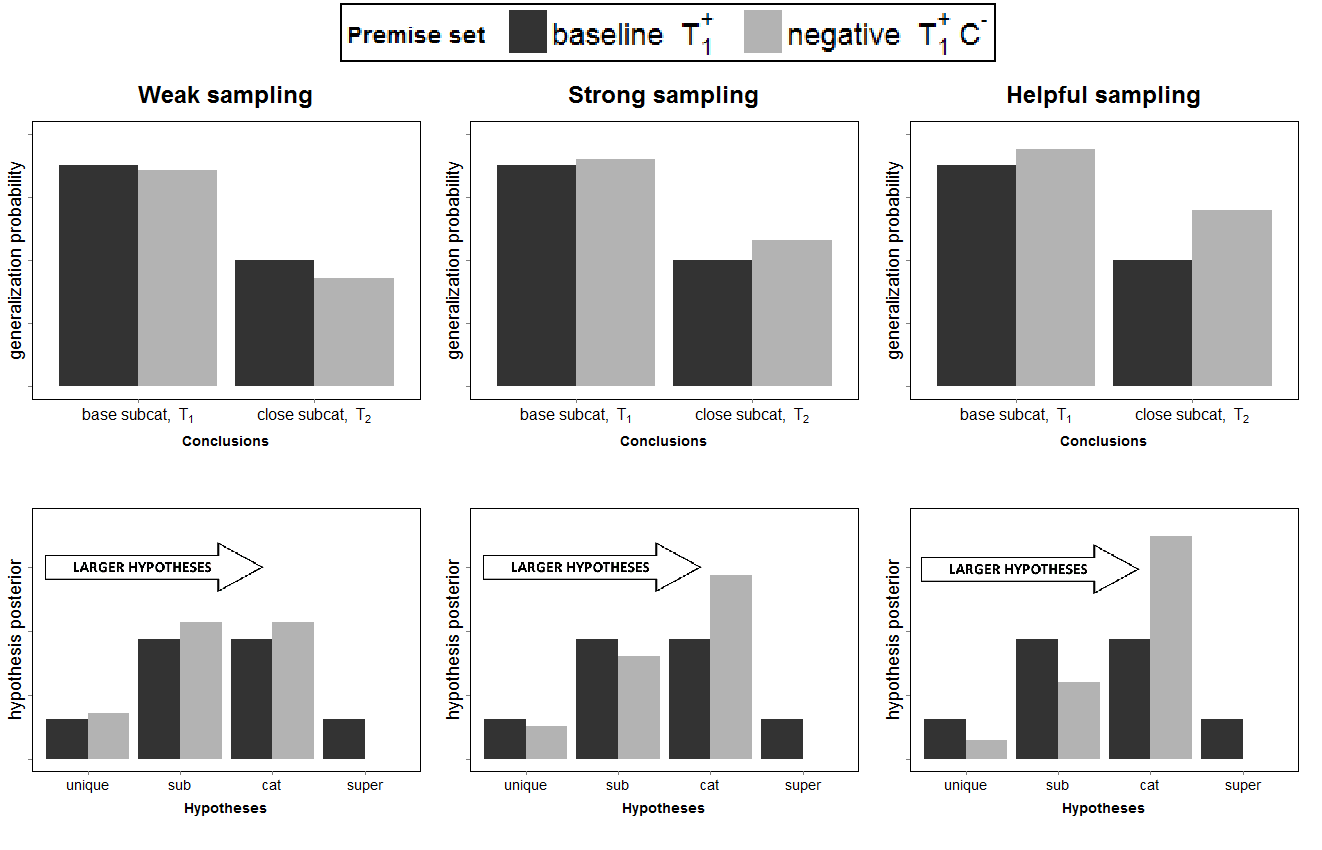
\includegraphics[trim = 2mm 0mm 7mm 0mm, clip,scale=.36]{fig/modelsimulations.png}
\vspace{-3mm}
\caption{Simulated results for inference in a simple domain with hierarchical structure like that in our experiments. The top row represents generalization probabilities to the same subcategory ({\sc base subcat, $T_1$}) and a different subcategory ({\sc close subcat, $T_2$}). This is analogous to learning that Mozart's music elicits alpha waves and giving generalization probabilities to Bach or Nirvana. Two premise sets are compared. The first, {\sc baseline} premise, is randomly sampled from the domain in all conditions. Analogously to our experiments, the second negative premise ({\sc negative}) comes from a different category in the domain: a falling rock does not elicit alpha waves. The panels differ in the sampling assumptions on how that premise was generated, growing more sophisticated from left to right: randomly from the domain (left), randomly from the set of possible negative observations (middle), or selected from the set of negative observations by a helpful teacher (right). The simulations reveal that more sophisticated sampling assumptions raise the probability of generalizing to a different subcategory when receiving the negative observation from a different category (top row). This is paralleled by an increased probability of the {\sc category} level hypotheses (bottom row).}
\label{fig:toys}
\end{figure}

Secondly, the success of the strong sampling model is surprising because it corresponds to a rather odd theory for the data. The ``random premise'' assumption in the weak sampling model is in some respects quite intuitive. The strong sampling model assumes that the negative premise is {\it required} to be negative, perhaps because a human constructing an argument has deliberately chosen to give a negative observation. But it also assumes that the negative observation is chosen {\it randomly} from the set of possible negative observations, which seems quite at odds with how people actually would construct arguments. Why would anyone construct an argument in this fashion, and why would any reasoner assume that an argument was constructed that way? Surely if a human communicator chooses to provide negative evidence, they will select negative evidence designed to be informative. In real conversations, people give information and construct arguments with a purpose in mind: an inductive argument is a speech act, designed to convince the reasoner or learner of the truth of some hypothesis about the world in an efficient and effective way. Clearly, just selecting at random from all possible negative observations does not serve that goal well. Moreover, the reasoner can be aware of the intention of the teacher, and use this ``model of the teacher'' to guide their inferences, e.g., by assuming that the negative observation is marking a boundary \citep{Levinson1995, SperberWilson1995}.

Inspired by theories about pragmatics in human communication \citep{Grice1989, Levinson1995, FrankGoodman2012} we propose an alternative to strong sampling, which can be referred to as {\it persuasive sampling} or {\it helpful sampling}. According to this theory of argument construction, the reasoner assumes that the premises have been assembled by another human who has chosen facts with the intent of helping them arrive at a particular conclusion in an efficient way. One way to quantitatively implement such a theory is to assume that the communicator selects evidence in a way that is tied to what they believe the reasoner will infer from that evidence \citep[see][]{Shaftoetal2014}. This is given by:

\begin{equation}
P(d^-|h) \propto P(h|d^-)
\label{eq:informative}
\end{equation}

\noindent In this equation, the probability that the communicator selects the negative observation $d^-$ given that their goal is to persuade the reasoner of hypothesis $h$ is proportional to the degree of belief that the reasoner would assign to hypothesis $h$ if data $d^-$ were provided. In its full generality this model creates a recursive relationship in which the communicator's evidence selection depends on the reasoner's beliefs and vice versa, and the actual likelihood function $P(d|h)$ is inferred by an iterative algorithm. We simplify this by running the algorithm for only one iteration, with an initial likelihood function specified by strong sampling. This corresponds to assuming that people's social reasoning relies on a one-step theory of mind (``the reasoner thinks that the communicator thinks that data $d$ are useful''; \citealp[see][]{GoodmanStuhlmuller2013, TesslerGoodman2014}).

In the light of how pragmatic and social assumptions might influence human inductive reasoning, the helpful sampling model seems much more sensible than strong sampling. If people think that an argument consists of purposeless and arbitrary facts, they should rely on a weak sampling assumption. But if they believe that an argument is constructed by a person for a reason, they should apply a helpful sampling theory, not a strong sampling one. In fact, many of the papers that have used strong sampling models have done so in situations where data are selected by helpful teachers, not situations where constrained-but-otherwise-random evidence is presented to people \citep[e.g.][]{xu_sensitivity_2007,gweon_infants_2010,Ransometalsubmitted}.

To what extent does this reliance on strong sampling models in place of more socially-inspired ones matter? To assess this, we simulated the results for our experiments using weak, strong and helpful sampling models. The details of the model structure and simulations are described in the Appendix. The simulation results, shown in Figure~\ref{fig:toys}, reveal that different sampling assumptions do lead to different generalizations and different beliefs in the manner described: the weak sampling model produces only modest belief revision when presented with negative evidence. It falsifies hypotheses at the {\sc superordinate} level, but this has almost no impact on the generalizations. The strong sampling model produces a more convincing pattern of results: in addition to falsifying {\sc superordinate} level hypotheses, it shifts its beliefs to favor the {\sc category} level hypotheses similar to humans. However, when we look at the model's generalizations, the increase for the $T_2$ item is very minor, and smaller than what is empirically observed (in Figures~\ref{fig:exp1me} and \ref{fig:Exp2_MainEffects}). In contrast, the helpful sampling model not only produces the right qualitative effect, the size of the effect is much larger and more in keeping with what human participants do.

In sum, our simulations suggest that the reason why people make non-monotonic generalizations from negative evidence has to do with the sampling assumption that they rely on in reasoning tasks. In the next section, we present an empirical test of this hypothesis by experimentally manipulating the sampling assumptions.

\section{Experiment 3}

In Experiments 1 and 2, participants were not given any context for the inductive arguments they were asked to assess. Without such context it is not unreasonable to think that people would assume a helpful sampling model. Indeed, this is exactly the kind of default assumption people are expected to make in most conversational contexts \citep{Grice1989, Levinson1995}, in which received information is taken to be relevant to the conversation. If so, the non-monotonic generalizations observed in the experiments are caused by the sampling assumption. This generates a testable prediction: if we supply participants with additional context that strongly suggests that the argument is constructed ``observationally'' by assembling true but otherwise arbitrary facts about the world, people should switch to a weak sampling assumption and the non-monotonic generalizations should vanish, as predicted in the left panel of Figure \ref{fig:toys}. This is the goal of Experiment 3.

\subsection{Method}

\subsubsection{Participants}
Participants were 200 workers from the United States on Amazon's Mechanical Turk (87 females), who participated for US\$0.60. The average age was 33.24.

\subsubsection{Materials}
People were presented with four arguments from four different topics ({\it music}, {\it fruit}, {\it animals}, and {\it types of water}), constructed in the same fashion as Experiments 1 and 2. Arguments in the {\sc baseline} premise set condition contained only a single positive observation taken from the base subcategory $T_1$. In the {\sc negative} condition an additional negative observation from a contrast category $C$ was included. Participants were asked to make generalizations to novel items from both the base subcategory $T_1$ and a different subcategory $T_2$. As with Experiment 2 we included four filler arguments and one initial argument to make sure they understood the task. Participants in different sampling conditions saw different filler items, designed to suggest different theories of the argument to participants (described below). Unlike Experiments 1 and 2 we did not include a hypothesis generation task, because we wanted to verify that the non-monotonic reasoning effects observed previously were not dependent on the inclusion of this task. Materials are presented in Table \ref{table:stimexp3}.

\begin{table}[t]
\scriptsize
\begin{center}
\caption{Stimulus material in Experiment 3. Each argument was presented with the {\sc baseline} premise and people were asked to generalize to the two conclusions. Depending on the condition, the second {\sc negative} premise was or was not included. The fillers were always presented with a second premise, a minus sign indicating it was presented as a negative premise. The example was presented in the instructions, and Trial 1 and 2 were the first two arguments presented to the participants. All other arguments were presented in random order.}
\label{table:stimexp3}
\vskip 0.12in
\begin{tabular}{|c|cc|cc|}
\multicolumn{5}{c}{\textbf{Experimental items}}\\
\hline
& {\sc baseline ($T_1$)} & {\sc negative ($C$)} & base subcategory, $T_1$ & close subcategory, $T_2$ \\
\hline
music & Mozart & -waterfall & Bach & Nirvana\\
fruit & strawberries & -blades of grass & blackberry & apple\\
animals & ducks & -elephants & swan & blackbird\\
types of water & Atlantic ocean & -tap water & Mediterranean & Lake Balaton\\
\hline \multicolumn{5}{c}{ } \\
\multicolumn{5}{c}{\textbf{Fillers (weak sampling)}}\\
\hline
& Premise 1 &  Premise 2  & Conclusion 1 & Conclusion 2 \\
\hline
Example & sheep & -dogs & horses & chickens\\
Trial 1 & aluminium & lead & copper & tin\\
Trial 2 & Earth & -weather satellite & Uranus & Sun\\
Filler & cobras & -iguanas & pythons & sea turtles\\
Filler & physicists & engineers & mathematicians & carpenters\\
\hline  \multicolumn{5}{c}{ } \\
\multicolumn{5}{c}{\textbf{Fillers (helpful sampling)}}\\
\hline
& Premise 1 &  Premise 2 & Conclusion 1 & Conclusion 2 \\
\hline
Example & sheep & cows & horses & pigs\\
Trial 1 & aluminium & -brass & copper & lead\\
Trial 2 & Earth & Mars & Uranus & Sun\\
Filler  & cobras & -pythons & vipers & anacondas\\
Filler & physicists & mathematicians & chemists & carpenters \\
\hline \multicolumn{5}{c}{ }
\end{tabular}
\end{center}
\end{table}


\subsubsection{Procedure}

Participants were presented with arguments related to all four topics, two of which included only the {\sc baseline} premise, and two were presented in the {\sc negative} condition (participants were randomly assigned to one of two versions, in which either the topics music and fruit were in the {\sc baseline} condition and animals and water in {\sc negative} or the other way around). On every trial, participants were first presented with the base premise. On the {\sc negative} evidence trials participants were then shown the second premise, but the way in which this information was delivered, depended on which sampling condition the participant was assigned to. After the premises were presented, participants were asked to judge the probability of two different conclusions, one related to an item from $T_1$ and the other from $T_2$ on a slider going from 1 to 100.

In order to encourage different sampling assumptions, there were two differences between conditions. The first manipulation related to {\it how} the negative evidence was presented. In the {\sc helpful sampling} condition, participants were told that the negative observation was generated by people in a previous experiment who had judged it to be helpful, in order to encourage people to adopt a helpful sampling assumption. In the \textbf{\sc weak sampling} condition people were asked pick a card from a deck of 49 cards presented face down on the screen, and were told that each card listed a randomly selected object fact related to the topic. They were shown the same information regardless of which card they picked: the point of the manipulation was to give people the impression that the negative evidence was generated more or less at random.

In addition to the different manner in which evidence was presented, we attempted to manipulate the sampling assumptions by giving people different filler arguments in the two conditions. In the {\sc helpful sampling} condition the second piece of evidence in the filler arguments was genuinely helpful and relevant.  In the {\sc weak sampling} condition, on the other hand, the additional information was designed to give a more random feel across the entire task: For at least one argument the extra information seemed rather irrelevant, and for the remaining arguments, the extra information did not  seem consistently helpful or particularly unhelpful. The use of different filler sets was necessary to make the different stories in each condition believable: the alternative would have been for people in the ostensibly random condition ({\sc weak sampling}) to consistently see premises that looked helpful, or for people in the {\sc helpful condition} to consistently see premises that looked random. For each participant the first two trials were fillers that supported that condition's story (see Table \ref{table:stimexp3}). The remaining six arguments -- four targets and two fillers -- were presented in random order.

\begin{figure}[t!]
\begin{center}
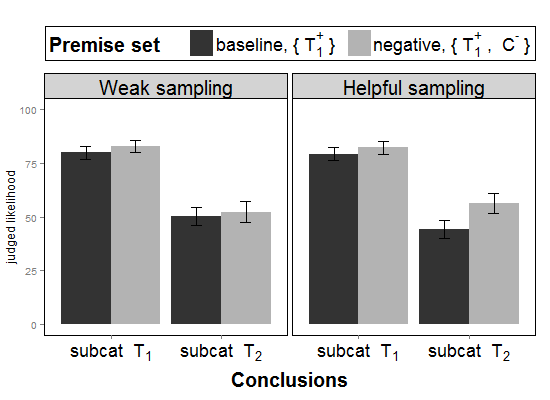
\includegraphics[scale=.5]{fig/exp3_gen_all.png}
\caption{Willingness to generalize to the novel members of the original subcategory $T_1$ or to a member of a different subcategory $T_2$ as a function of sampling condition. Error bars show the 95\%CI. As predicted, people showed non-monotonic generalization in the {\sc helpful sampling} condition (left) but not the {\sc weak sampling} condition (right). When they thought the negative observation was generated by a helpful person, they increased their generalization to a different subcategory, but they did not do so when the negative observation was randomly sampled from the domain.}
\label{fig:exp3_me}
\end{center}
\end{figure}

\subsection{Results \& Discussion}

The critical prediction relates to people's generalizations to members of subcategory $T_2$. An effect of premise set was expected in the {\sc helpful sampling} but not the {\sc weak sampling}, and as Figure~\ref{fig:exp3_me} demonstrates, the predicted pattern is precisely what was observed. In the {\sc helpful sampling} condition, the negative evidence encouraged people to generalize more broadly (Cohen's $d$ = .41, BF = 776:1), whereas in the {\sc weak sampling} condition no such pattern exists (Cohen's $d$ = .07, BF = 7:1 in favor of the null). In other words, the role that negative evidence plays in inductive reasoning genuinely does seem to be shaped by the sampling assumptions people rely on, and these assumptions can be manipulated by changing the context in which the argument is presented.

\section{General Discussion}

Most research on inductive inference has focused on the effects of positive observations. Although the question is very similar, disproportionately little attention has been paid to how negative observations influence inference. This is remarkable, not least because negative observations are encountered far more frequently: most things in the world are non-edible, not-dangerous, not-animals, and so forth (see \citealt{KalishLawson2007}). Admittedly, the reasonable assumption that positive observations are rare is thought to be one of the reasons people attribute more weight to them over negative observations  \citep{McKenzieMikkelsen2007} and have a general bias towards strategies that involve positive tests \citep[e.g.][]{NavarroPerfors2011, OaksfordChater1994}. Yet, given the sheer frequency of negative observations, whether implicit or explicit, it is imperative to more deeply understand how they can guide inference.

Our work makes two main contributions. First, we showed that in hierarchically structured domains, negative observations can raise the willingness to generalize to other items. This contradicts the overall pattern of a monotonic relation between the sign (negative or positive) of an observation and its effect. We found that the effect is most detectable in generalizations to objects of intermediate similarity to a base premise -- this was evident in generalizing from Mozart to Nirvana given that falling rocks do not have the property. Generalizing from Mozart to Bach given that Metallica doesn't have the property is structurally identical but did not show the same pattern in our data; this was probably because of a ceiling effect due to the high existing similarity between Mozart and Bach dominating the inference.

Second, closer examination of the types of hypotheses participants generated, suggested that negative observations produce this effect by drawing belief to the largest remaining hypothesis, pulling belief from the smaller hypotheses. This transfer effect is essential for non-monotonic generalization, and is inconsistent with any form of belief updating that simply falsifies incorrect hypotheses, such as Bayesian weak sampling. It {\it is} consistent, however, with more sophisticated assumptions on part of the reasoner about how the observations were selected: if she assumes that the negative observation was chosen from the set of possible negative observations, a shift in belief from smaller to larger consistent hypotheses is sensible. This belief shift becomes especially pronounced when the reasoner operates on the assumption that the negative evidence has been deliberately chosen to be informative, helpful and relevant. We presented modeling results that explain this effect, and Experiment 3 experimentally confirms it: non-monotonic generalization emerged in a helpful sampling scenario, but not in a weak sampling scenario.

Given the results of Experiment 3, why did participants in Experiments 1 and 2 generalize non-monotonically? After all, the first two experiments gave no explicit indication about how the arguments were constructed. The most plausible answer is that people thought -- probably sensibly -- that the experimenter was providing them with information relevant to the problem at hand. That is, their natural theory about how the premise sets were constructed was that they were provided by a helpful teacher. In hindsight, it may not come as a surprise that a weak sampling scheme was not the default assumption in our category-based induction tasks. There is widespread evidence that human interlocutors and learners often assume stronger forms of sampling \citep{SanjanaTenenbaum2003,Vanderhenstetal2002, XuTenenbaum2007}, in particular in communicative \citep{GoodmanStuhlmuller2013} and pedagogical contexts \citep{Shaftoetal2014}. These assumptions influence the inductive inference process, as we found here (see also, \citealt{Fernbach2006, LawsonKalish2009, Navarroetal2012, Vanderhenstetal2002cogsci, Vongetal2013, Shaftoetal2014, Ransometalsubmitted}).

From a pragmatic perspective, it is in fact expected that participants would make the assumption that the experimenter is trying to be cooperative -- an assumption that is the default in most human communication contexts \citep{FrankGoodman2012, Grice1989, Levinson1995}. This tremendously facilitates both communication and learning: thinking the other is trying to be as informative as possible increases one's degree of belief change \citep{SperberWilson1995}. The cooperative communicator is expected to pick a particular observation, and not another, because she realizes which inferences these observations will provoke in the hearer; the hearer can, accordingly, revise their belief in bolder ways by considering that particular observation to be relevant and maximally informative. Of course, what {\it exactly} is relevant and maximally informative depends on the common ground communicators share and effective reasoning depends on the ability to accurately model the other persons' prior assumptions. Our experiments involved domains in which people generally already know the structure and have sensible prior assumptions and this structure was very visible in the argument; the extent to which the assumption of helpfulness matters in less well-understood domains remains an open question.

Interestingly, our analysis implicitly points to the importance of the alternative negative observations that were available to to the teacher to choose from. Indeed, in our Bayesian model, helpfulness is closely related to the choice of a particular negative observation in the light of possible alternatives. Confronted with the information that the sound of a waterfall does not elicit alpha waves, a learner could still have substantial belief in the hypotheses that music or classical music is the true feature extension. But precisely because the learner expects the teacher to choose a negative observation closer to classical music if that were the true hypothesis -- e.g., Metallica does not elicit alpha waves -- a more dramatic belief revision takes place in favor of the all-music hypothesis. Perhaps not surprisingly, this is consistent with the role of alternatives in other communicational phenomena that are typically studied from a pragmatic perspective, such as scalar implicatures and horn implicatures \citep[e.g.][]{Barneretal2011, Bergenetal2012, Chierchiaetal2001, SullivanBarner2011, Stilleretal2011}.

\subsection{Non-monotonicity in category-based induction}

Non-monotonic generalization does not emerge only when given negative observations. Violations in which positive observations lower conclusion likelihood have also been found. For example, suppose people are asked to judge how likely it is that goats have some property X. They will be more willing to endorse the conclusion when told that brown bears have property X than when told that brown bears, black bears and polar bears have property X. Despite the additional positive observation in the latter circumstance, generalization judgments are lower \citep{Medinetal2003}. The non-monotonicity in our experiments is the inversion of that effect: in the positive case a reasoner's generalization ``tightens'' to a small subcategory by introducing an positive observation that is very similar to the base premise. The negative observation ``expands'' generalizations to larger categories.

In related research in our lab, and building on work by \citet{Fernbach2006}, we have been studying how non-monotonic generalization following positive observations can be captured in a way similar to the one proposed here \citep{Ransometalsubmitted}. If a learner assumes that the bears in our example are sampled from the correct hypothesis (that is, strongly sampled), it is rational to infer that only bears were sampled because the correct hypothesis is that all bears (and only) bears have the property: why would a teacher present only bears if that were not the correct hypothesis? In contrast, if the learner believes the observations are randomly encountered, a hypothesis that is about bears does not gain relative probability -- seeing three bears as premises is simply (really) bad luck that she did not encounter something more informative.

\subsection{Implications for models of induction}

At a general level, our findings do have two clear implications for the theoretical understanding of category-based induction. First, our results suggest that the conceptual structure underlying a domain influences inferences in specific and sometimes surprising ways. Non-monotonic generalization emerges when hypotheses are hierarchically structured -- that is, the hypotheses are nested within and do not cross-cut one another. Second, we have shown that generalization is driven in part by the assumptions people make about how premises are  sampled. This is line with recent findings in other generalization tasks. For example, Shafto and colleagues \citep{ShaftoGoodman2008, Shaftoetal2014} have shown that when learners have to guess the size and position of a rectangle in a grid, they will expect teachers to provide them with positive observations in the corner of the unknown rectangle (thus determining the size and position) and negative observations marking the borders of the rectangles, and they infer size and position accordingly. When they (randomly) select observations themselves, they will not consider these observations to be in the corners or marking the borders, leading to different, more uncertain inferences. While such effects of sampling assumptions can be implemented in various ways at a process level, it is clear that any model of category-based induction should have some way of capturing them.

The observation of non-monotonicity and the influence of sampling assumptions, present a challenge for the similarity-based approach that is commonly found in models of category-based induction. On the basis of similarity, one would expect strictly monotonic generalization. To save similarity as an explanatory principle, however, one could argue that a more flexible and context-dependent notion of similarity can account for our findings (see, e.g., \citealt{Medinetal1993}). Indeed, the addition of a particular premise may enhance similarity between the first premise and a conclusion, facilitating the generalization, and thus -- in case the additional premise is negative -- lead to the observed non-monotonicity. But even then the similarity approach would struggle with the results of Experiment 3, as assumptions about how the premises were generated are not a natural component of such an approach. This raises questions about the extent to which modifications to the similarity approach would be necessary to explain these results\footnote{In fact, one could recast the similarity approach in a Bayesian framework (following \citealt{TenenbaumGriffiths2001}), which would allow the specification of sampling assumptions through the likelihood function. The result would be a model that is identical to the one discussed here. This equivalence points to the, perhaps not yet exhaustively understood, relatedness of similarity, generalization and categorization.} and the extent to which existing models can be modified to predict non-monotonicity and the effect of sampling assumptions (see also \citealt{Heussenetal2011} for a more detailed overview). The same holds for numerous other phenomena involved in category-based induction, since the existing models are good at capturing some effects and have difficulties with others (see, e.g., \citealt{Hayesetal2010}, for a review).

Perhaps the most natural perspective for explaining the present findings is the relevance theory of induction \citep{Medinetal2003} which builds on key insights from the Gricean analysis of communication and in a way acknowledges a more flexible notion of similarity as well as the role of sampling assumptions. According to relevance theory, every act of communication carries in itself the presumption of its own relevance, and people will try to interpret it in a way that maximizes relevance, that is, results in a maximum cognitive effect \citep[e.g.][]{Vanderhenstetal2002}. In category-based induction, the relevance principles have proven useful in the analysis of certain phenomena such as non-monotonicity with positive observations \citep{Medinetal2003}, processing times of premises and their associated effect on belief revision \cite{Feeneyetal2010}. Applied to the present findings, relevance theory would argue that the addition of a negative observation from a different category reinforces the relevant feature shared by the base premise and the conclusion category. In order to maximize the effect that a negative observation has on inference, it is interpreted as pointing to the largest hypothesis still consistent with the premise and the conclusion.

This analysis aligns readily with the Bayesian analysis we have presented earlier. However, our work builds on and strengthens it in several important ways. One of the main arguments against relevance theory is that the core concept of relevance is notoriously slippery and lacks predictive power. Indeed, there is a sense in which relevance is defined in a circular manner: a feature is relevant because it leads to a large cognitive effect, and it has such effect because it is relevant. Our computational analysis of the present findings is substantially more systematic and precise. Firstly, we have shown {\it why} one particular feature (and not another) can be reinforced when adding a negative observation, in demonstrating that under strong sampling assumptions, larger hypotheses (features) are favored. Secondly, we have illustrated that the extent to which the feature is reinforced further depends on the assumed relevance of the observation, that is, whether the learner thinks it was intended to be helpful or not. As category-based induction experiments often evoke a social context, and participants implicitly expect the information they receive to be informative for the inductive problem \citep[e.g.][]{Medinetal2003}, the further reinforcement also emerges in context where the usefulness is not explicitly acknowledged.

Our results join a growing body of research suggesting that the pragmatic context in which information is presented to people has the potential to dramatically alter the inferences they are willing to make. This also has clear consequences for further empirical investigations. We as experimenters should be aware that different tasks can imply different pragmatic contexts for participants, and this in turn can result in different generalization patterns. It is therefore vital to thoroughly consider the specification of that context. Indeed, although infamously stubborn, given the appropriate pragmatic context even Zeno may eventually have been convinced that kangaroos can, in fact, outrun tortoises. Perhaps even by the argument that a rock cannot. Not even on a windy day.

\section{Acknowledgements}

WV is a postdoctoral researcher at the Research Foundation -- Flanders. DJN received salary supported from ARC grant FT110100431 and AP from ARC grant DE120102378. Initial versions of this work were presented at the 35th Annual Conference of the Cognitive Science Society. We thank Chayenne van Meel for help with the experiment construction and data collection of Experiment 1 and Daniel Heussen for fruitful discussion.

\section{References}

\bibliographystyle{model5-names}
\bibliography{lit/negev}


\appendix

\section*{ Appendix: Computational model simulation}

Our model simulation relies on two crucial components. First, the specification of the hypothesis space and second, the specification of the likelihood function used to update beliefs and make inferences following an observation. We will describe both components in more detail.

\subsection*{Hypothesis space}
The model simulations presented in this paper are based on an abstract, simplified representation of the hypothesis space of participants. In particular, we assume that the types of hypotheses the participants are considering directly map onto the hierarchical structures as depicted in figures \ref{fig:exp1_itemstruc} and \ref{fig:exp2_itemstruc}. Using music as an example, the space consists of the hypotheses that project the property to the relevant singleton (e.g., Mozart's music) or to any subset of items that share the same knot in the tree structures (classical music, rock music, music, nature sounds, all sounds).

The prior probability of the hypotheses was set to be relatively uninformative, with lower belief in ``extreme'' hypotheses, singletons and the all-encompasing hypothesis (all sound). In total, we simulated the domain of sound as having 100 items, with music comprising 50 items and nature sounds 40 items. Rock music and classical music each contained 10 items. Details for the hypotheses are presented in Table \ref{table:Hsettings}.

\begin{table}[H]
\begin{center}
\scriptsize
\caption{\small Specifications of the relevant hypotheses, priors and hypotheses size used for the model simulations. Updates are also presented for the {\sc baseline} premise set (Mozart has X) and the three sampling schemes for the negative observation in the {\sc negative} premise set (the sound of a falling rock does not have X).\normalsize}
\label{table:Hsettings}
\begin{tabular}{lcc||c|ccc}
\hline
hypothesis & size & prior & {\sc baseline} &\multicolumn{3}{c}{{\sc negative}}\\
& & & & Weak sampling & Strong sampling & Helpful sampling \\
\hline
Mozart's music & 5 & .07  &.13	&	.14	&.10	&.06	\\
classical music & 10 & .21&.38	&	.43	&.32	&.24	\\
rock music & 10 & .21			&0 		&	0		&	0		&0\\
music & 50 & .21					&.38	&	.43	&	.58	&.70\\
nature sounds & 40 & .21	&0		&	0		&	0		&0\\
sound & 100 & .07					&.13	&	0		&	0		&0\\
\hline
\end{tabular}
\end{center}
\end{table}

\subsection*{Making inferences}

We evaluated the equivalent of following argument, corresponding to premise set {\sc negative} in our experiments:

\MyQuote{Mozart's music elicits alpha waves in the brain\\
The sound of a falling rock \textbf{does not} elicit alpha waves in the brain\\[-5pt]
\rule[0pt]{250pt}{1pt} \\[-2pt]
Nirvana's music elicits alpha waves in the brain
}

Crucially, we compared the probability of the conclusion following the premise without the second negative observation to the probability of the conclusion following the premise set with the negative observation. The model output for the probability that a particular item, $y$, the conclusion, is a member of the true extension of a feature, $f$, given an observation $d$ (a premise) was calculated by:

$$P(y \in f|d)=\sum_{y,d\in h}{P(h|d)}$$

\noindent
where $h$ refers to the hypotheses that people entertain regarding the true extension $f$. The probability of an hypothesis given an observation is given by Bayes' rule (see Equation \ref{eq:bayes}), which hinges on the specification of the likelihood function. We considered a weak sampling likelihood, a strong sampling likelihood and a helpful sampling likelihood.

For the two-premise argument, we sequentially updated the probability of hypotheses: First, the model observes that ``Mozart's music has X'', and hypotheses are updated accordingly. Then, the resulting posterior across hypotheses was updated a second time when the model observes that ``the sound of a falling rock does not have X''. For the first premise, we always updated using weak sampling, and for the second (negative) premise, the sampling scheme was either weak, strong or helpful.

\subsubsection*{Weak sampling}

In the weak sampling scheme, the model assumes that the observation was sampled randomly from the domain. By consequence, each observation is considered equally likely. Hypotheses that are inconsistent with the observation are excluded and relative differences in belief between hypotheses are maintained.

\subsubsection*{Strong sampling}

In this scheme, the model assumes that the observation is sampled from the hypotheses. Applied to negative observations, this means that the model assumes the observation was sampled from the complement of the true hypothesis, and beliefs are updated using the likelihood function specified in Equation \ref{eq:negstrong}.

\subsubsection*{Helpful sampling}

In this more sophisticated likelihood function, the probability of selecting a negative observation given a particular hypothesis, depends on the effect it is expected to have on the beliefs, as per equation \ref{eq:informative}. Obviously, to calculate the likelihood, an initial update is required, which requires a likelihood function, and thus Equation \ref{eq:informative} expands to:

$$
P(d^-|h) = \frac{\left( \frac{P(d^-|h)P(h)}{\sum_{h'}{P(d^-|h')P(h')}} \right)^{\alpha} }
{\sum\limits_{d'^-}{\left( \frac{P(d'^-|h)P(h)}{\sum_{h'}{P(d'^-|h')P(h')} } \right)^{\alpha} } }
$$

\noindent
To calculate this expression the ``initial'' likelihood, $P(d^-|h)$ is required, and is specified in Equation \ref{eq:negstrong} (strong sampling). For all simulations, we set $\alpha$ at 1. This parameter can be considered a quantification of helpfulness: larger values of $\alpha$ lead to stronger inferences on the basis of an increasingly ``helpful'' assumed likelihood function. As such, a larger $\alpha$ would magnify the non-monotonic generalization observed in Figure \ref{fig:toys}.

\subsection*{Robustness}

As explained in section 1.2 of this paper, under a strong sampling scheme negative observations will always favor larger hypotheses. This, however, does not necessarily mean that generalization to a particular object $y$ will rise after seeing the negative observation $d^-$, as the generalization requires summing across all hypotheses consistent with $d^-$ and $y$. Clearly, this makes sense, as we do not want our model to predict that a negative observation will always lead to non-monotonic generalization.

It is useful to explore the conditions under which non-monotonic generalization in a Bayesian framework can be observed. To identify the crucial conditions, let's consider the simplest case, that is, the hierarchical hypothesis space illustrated in Table A4, and considering generalization to Nirvana's music after having observed that Mozart has the property (the {\sc baseline} column). This leaves four nested hypotheses: assume $h_1$ is Mozart's music, $h_2$ is classical music, $h_3$ is music and $h_4$ is sound. If we consider the {\sc baseline} as the starting point, non-monotonic generalization to $y$ (Nirvana's music) after observing $d^-$ (the sound of a falling rock does not have the property) is defined as:

$$P(y \in f) < P(y \in f|d^-)$$

\noindent If we expand both sides of the inequality, this leads to:

$$\sum_{y \in h'}P(h') < \sum_{y \in h'}{\frac{P(d^-|h')P(h')}{\sum\limits_{h''}{P(d^-|h'')p(h'')}}}$$

\noindent If we then take into account that $y \notin h_1, h_2$ and $d^-$ is not consistent with $h_4$:

$$P(h_4) < P(h_3|d^-) - P(h_3)$$

Thus, non-monotonic generalization to $y$ (Nirvana's music) can be observed when the hypotheses that are falsified by $d^-$, in this case $h_4$, have smaller prior belief than the increase in belief for the hypotheses consistent with $y$ and $d^-$, in this case $h_3$. In words, the loss in willingness to generalization due to falsifying that all sounds have the property, should be smaller than the gain due to an increase in belief that all music has the property.

So, which factors drive this inequality, given the hierarchical hypothesis space? First, the more belief one has in the largest hypothesis ($h_4$) prior to observing $d^-$, the harder it is to satisfy the inequality. Second, relative to all hypotheses consistent with $d^-$, the hypotheses also consistent with the conclusion should gain disproportional support from $d^-$, to the extent that the increase outweighs the loss in belief from falsifying $h_4$. This condition is satisfied if $P(d^-|h_3)$ is relatively and sufficiently large in the combined likelihood of all remaining hypotheses ($h_1$, $h_2$ and $h_3$). This underlies the success of the strong sampling approach, as larger consistent hypotheses will yield a larger likelihood. To observe non-monotonic generalization, the size of $h_3$ should be sufficiently large compared to the smaller hypotheses $h_1$ and $h_2$, as the likelihood depends on the hypothesis size. Third, in helpful sampling, the helpfulness parameter $\alpha$ actually exacerbates differences in likelihood due to hypothesis size, and higher values of $\alpha$ thus facilitate the non-monotonic generalization in the strictly hierarchical domain.

\end{document}
